\documentclass[a4paper, 12pt]{scrartcl}

\usepackage{scrpage2}
\usepackage[left=2.5cm,right=2.5cm, top=3cm, bottom=4cm]{geometry}
\usepackage[utf8]{inputenc}
\usepackage[ngerman]{babel}
\usepackage[T1]{fontenc}
\usepackage{amsmath}
\usepackage{amssymb}
\usepackage{amsfonts}

\usepackage{graphicx}

\usepackage{float}
\usepackage{adjustbox}
\usepackage{hyperref}
\usepackage{textcomp}

%\usepackage{enumerate}
\usepackage[shortlabels]{enumitem}

% Einrücken verhindern
\setlength{\parindent}{0em} 


\begin{document}


\begin{titlepage}
	\centering
	{\Huge\bfseries Versuchsprotokoll\par}
	\vspace{2cm}
	{\scshape\LARGE Akustik \par}
	\vspace{1cm}
	{\Large Schallgeschwindigkeit in Festkörpern und die Physik der Gitarre\par}
	\vfill
	{\large\itshape Simon Schwarz und Marius Ising\par}

	\vfill
\end{titlepage}

\tableofcontents
\newpage

\section{Schallgeschwindigkeit in Festkörpern}


\subsection{Versuchsbeschreibung}

Das Ziel des folgenden Versuchs ist die Bestimmung der Schallgeschwindigkeit und des Elastizitätsmoduls von vier verschiedenen Metallen. Das Elastizitätsmodul 
$$E = \frac{F/A}{\Delta L/L}$$
ist eine Materialkonstante und gibt die relative Längenausdehnung in Abhängigkeit von der angreifenden Zugspannung an. Eine Messung ist über die Ausbreitungsgeschwindigkeit 
$$v_l = \sqrt{\frac{E}{\rho}}$$
möglich, wobei $\rho$ die Dichte des Materials bezeichnet. Die dynamische Bestimmung von $E$ durch das direkte Messen der Längenausdehnung ist bei Metallstäben nicht praktikabel, da für Metalle $E$ in der Größenordnung $10^{11} N/m^2$ liegt. Der Metallstab hat als Zylinder mit Länge $L$, Durchmesser $D$ und Masse $M$ die Dichte
$$\rho = \frac{4M}{\pi LD^2}\text{,}$$
so dass sich mit
$$v_l = 2L f_0$$
das Elastizitätsmodul
$$E = 16 f_0^2 LM \frac{1}{\pi D^2}$$
ergibt. Dabei ist $f_0$ die Grundfrequenz der longitudinalen Schallwelle, die neben den Größen $L$, $D$ und $M$ experimentell bestimmt werden soll.

\subsection{Versuchsaufbau}

Folgende Geräte werden für den Versuch benötigt: Zwei Tischklemmen, eine Kreuzmuffe, eine Metallstange $\sim 20$ cm, ein Metallstift, ein Metallstift, ein Sensor-Cassy mit Laptop, ein Mikrofon, ein Gummihammer, eine Waage, ein Bandmaß, eine Mikrometerschraube und vier Metallstangen $\sim 130$cm (Kupfer, Stahl, Aluminium und Messing).

\begin{figure}[h]
	\centering
	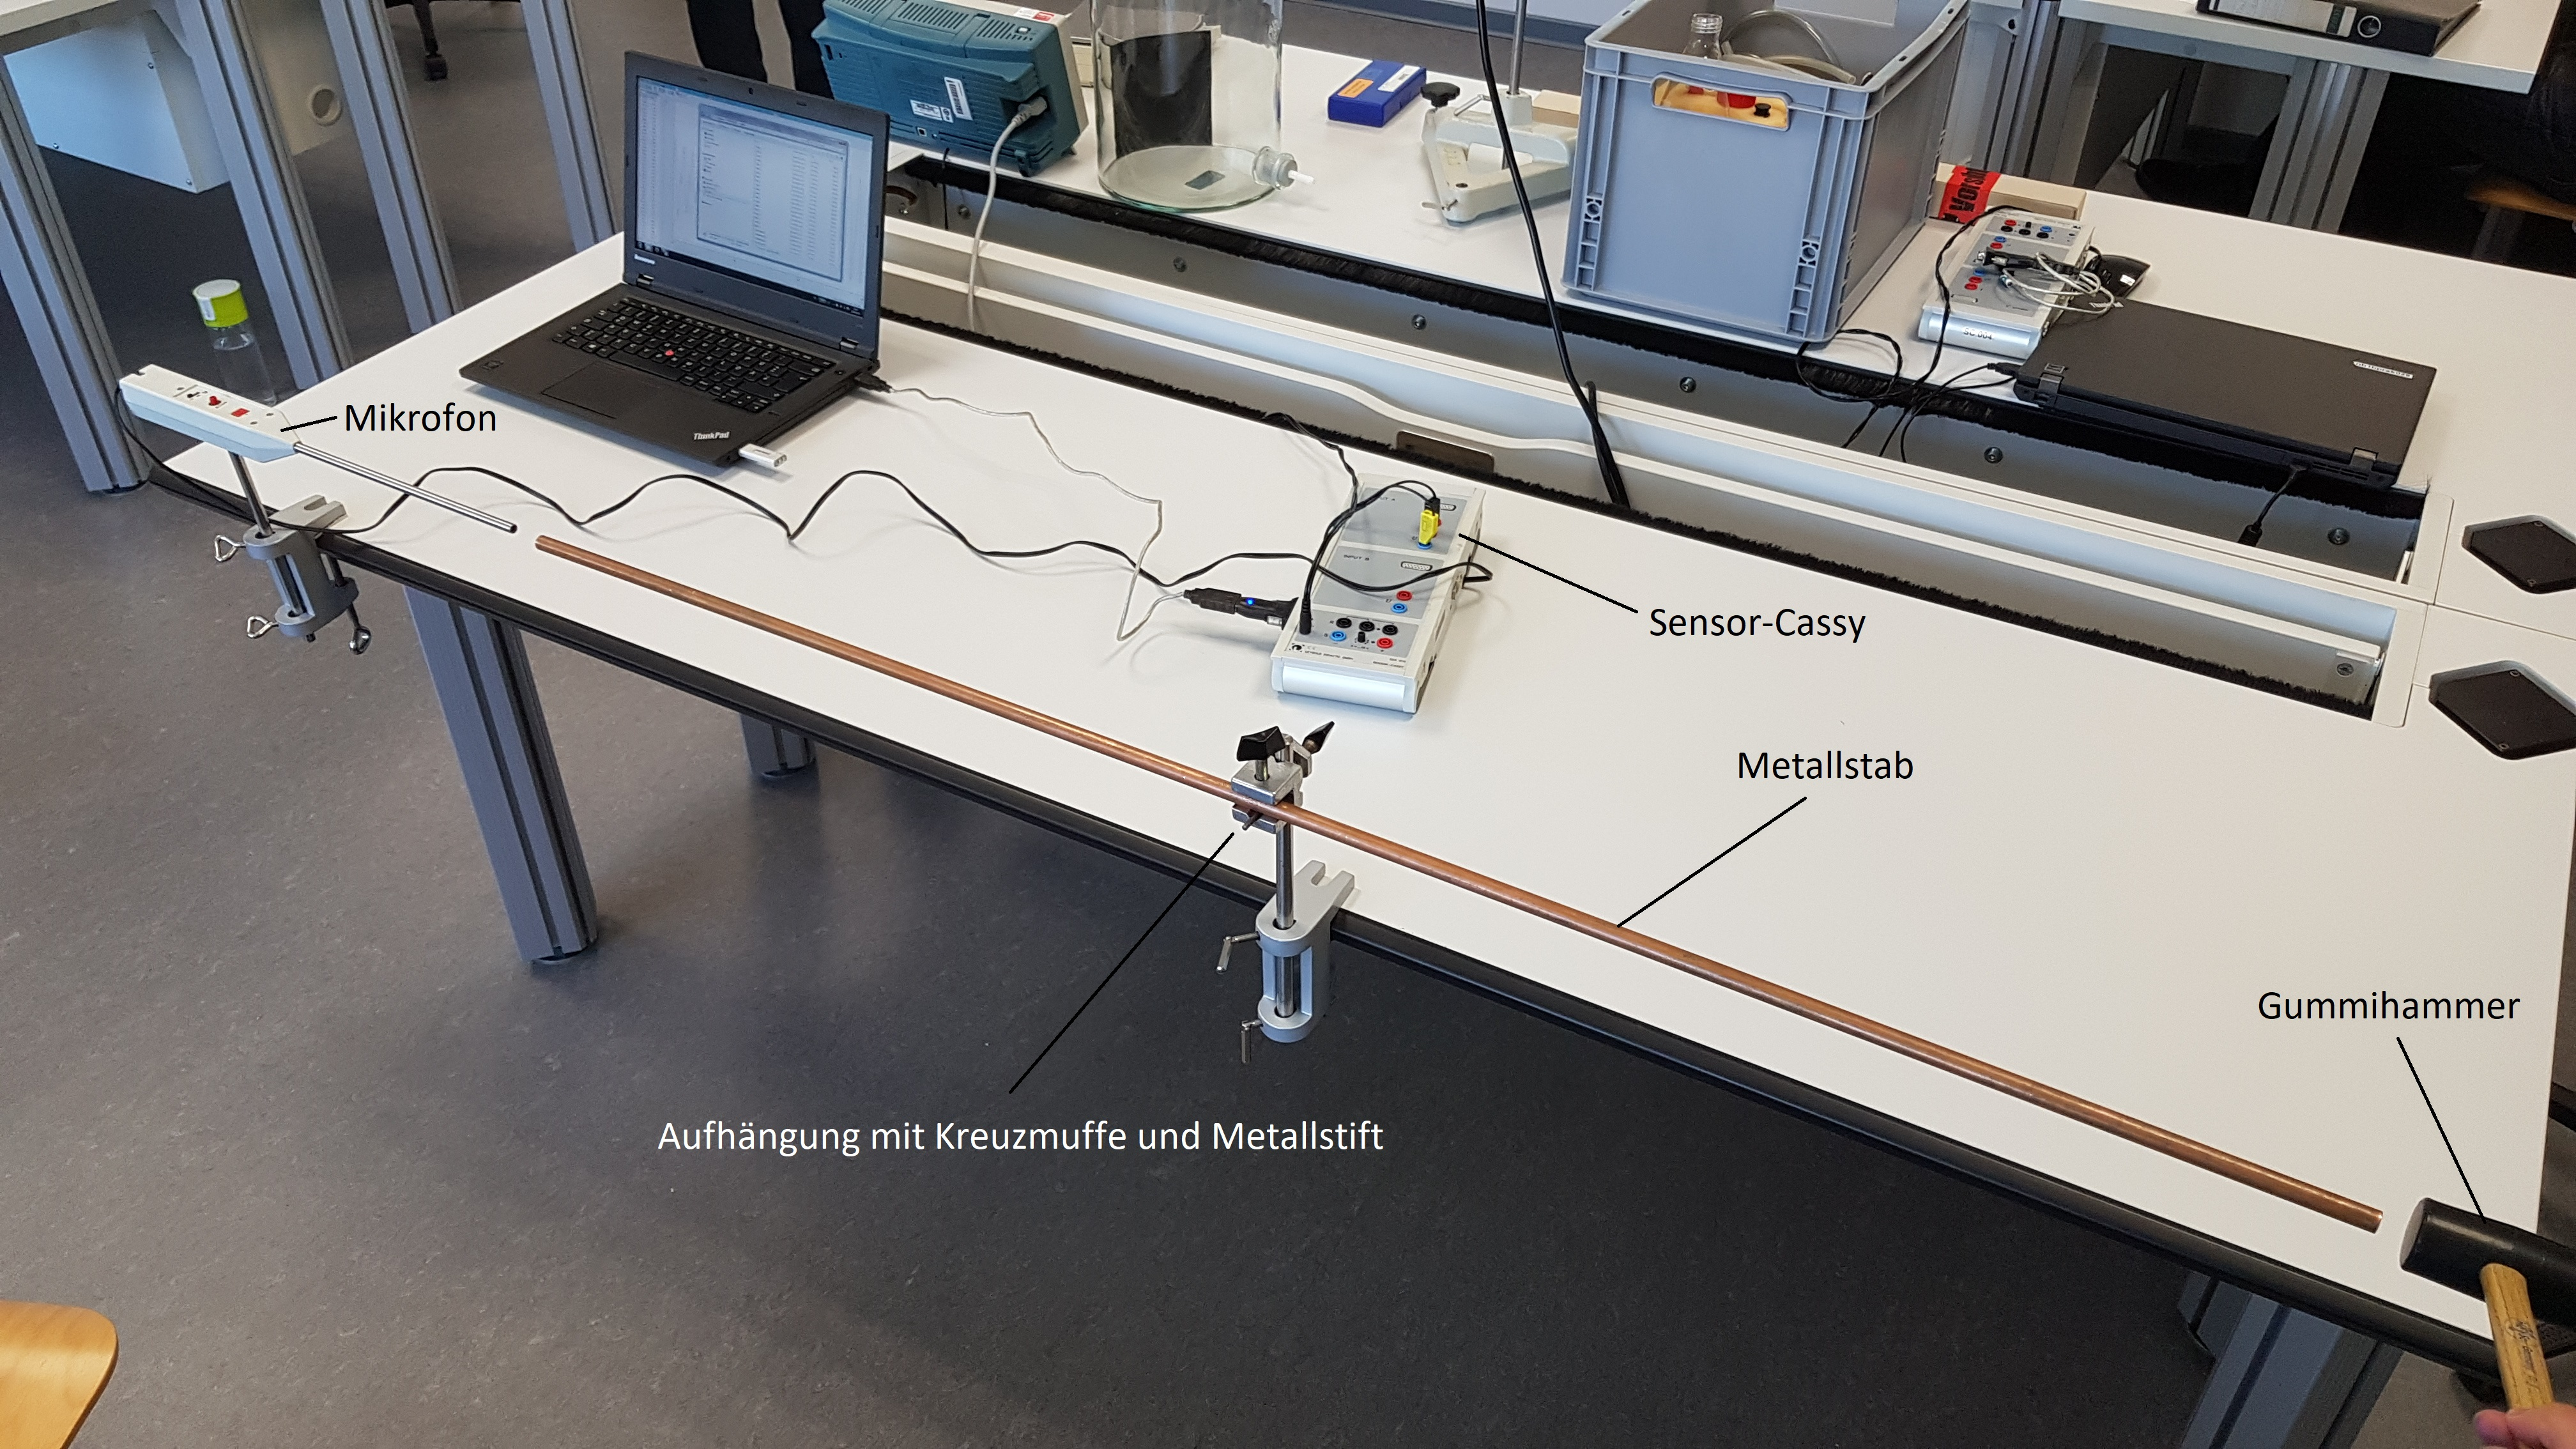
\includegraphics[width=\linewidth]{bilder/aufbau_festkoerper.jpg}
	\caption{Versuchsaufbau}
\end{figure}

Eine große, zu untersuchende Metallstange wird mit Hilfe einer Tischklemme, der kleinen Metallstange und der Kreuzmuffe horizontal am Tisch befästigt. Dabei muss die Stange mittig an zwei Punkten eingespannt werden, damit die Schwingung nicht beinträchtigt wird. Dies ist in Abbildung TODO dargestellt. In kleinem Abstand zu einem Ende der großen Metallstange wird das Mikrofon platziert, das den Schalldruck und somit die Schallwellen misst. Das Mikrofon ist am Sensor-Cassy angeschlossen. Am anderen Ende kann die Stange durch einen Schlag mit dem Gummihammer in Schwingung versetzt werden. Der Schlag sollte möglichst gerade auf das Ende der Stange erfolgen, um transversale Schwingungen des Stabes zu vermeiden.

\begin{figure}[h]
	\centering
	%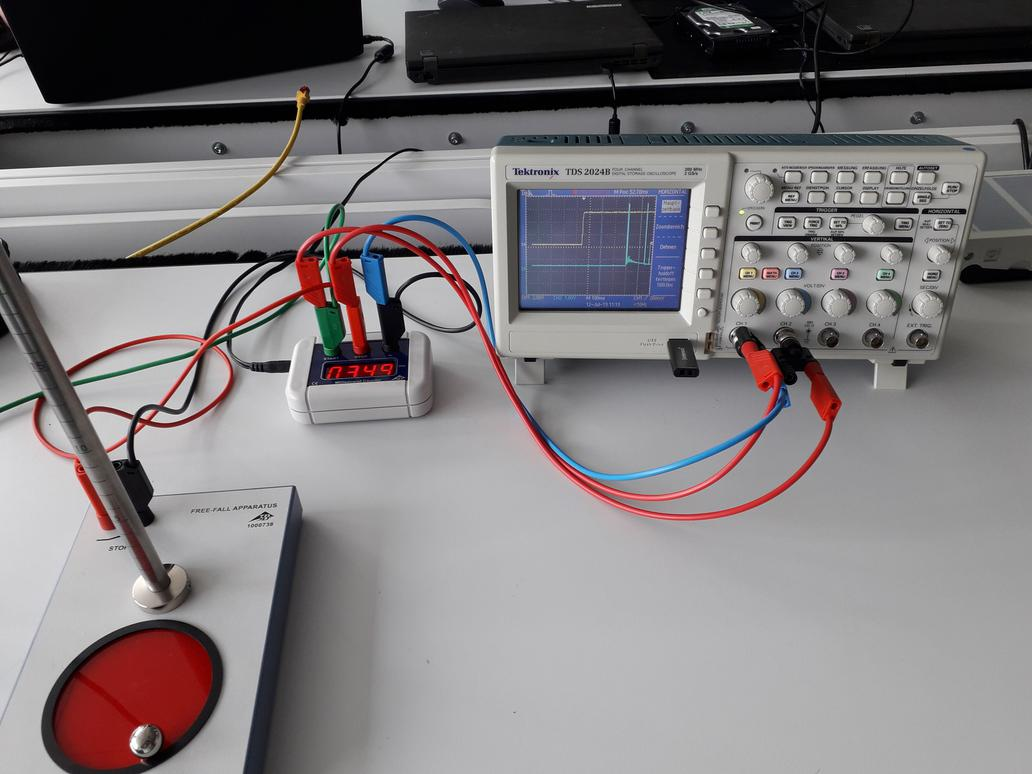
\includegraphics{bilder/Aufbau_Detail_ff.jpg}
	\caption{Anschluss von Digital-Zähler und Oszilloskop}
	\label{AnschlussOsDz}
\end{figure}



\subsection{Versuchsdurchführung}

Die Fallzeiten werden für verschiedene Höhen von 10 bis 90 cm in Schritten von 10 cm durchgeführt. Dabei werden für jede Höhe 10 Zeitmessungen mit dem Digitalzähler und eine Messung mit dem Oszilloskop durchgeführt. Das Oszilloskop wird dabei auf Single Seq eingestellt und auf die steigende Flanke des Startsignals getriggert. Das Triggerlevel liegt dabei bei 620 mV. Um eine Startgeschwindidkeit der Kugel zu vermeiden, wird der Auslösebügel möglichst feinfühlig betätigt. Es werden stets alle Messungen für eine Höhe durchgeführt, ehe die Höhe verstellt wird. Bei der Höheneinstellung wird versucht mit der oberen Bohrungskante der Startkonsole genau den Strich der Säulenskala zu treffen.


\subsection{Versuchsauswertung}

\subsubsection{Messung mit dem Digitalzähler}

Für die Höhenmessung ist entscheidend mit welcher Genauigkeit man den Skalenstrich trifft. Dabei wird die Unsicherheit auf $\sigma_s = 1 \, \mathrm{mm}$ geschätzt. Mit dem Digitalzähler ergaben sich die Messsungen aus Tabelle \ref{tableDz}.

\begin{table}[h]
\begin{center}
\begin{tabular}{c|r|r|r|r|r|r|r|r|r}
$s$ / cm & 10 & 20 & 30 & 40 & 50 & 60 & 70 & 80 & 90 \\
\hline
$t$ / ms & 140 & 200 & 245 & 284 & 318 & 348 & 376 & 403 & 427 \\
         & 140 & 200 & 246 & 284 & 318 & 348 & 377 & 403 & 427 \\
	 & 140 & 200 & 246 & 284 & 318 & 348 & 376 & 403 & 427 \\
	 & 141 & 200 & 246 & 284 & 318 & 348 & 377 & 403 & 427 \\
	 & 141 & 200 & 246 & 284 & 318 & 348 & 377 & 402 & 407 \\
	 & 141 & 200 & 245 & 284 & 318 & 348 & 376 & 402 & 427 \\
	 & 141 & 200 & 246 & 284 & 318 & 348 & 376 & 402 & 427 \\
	 & 141 & 200 & 245 & 284 & 318 & 348 & 376 & 402 & 427 \\
	 & 141 & 200 & 245 & 284 & 318 & 348 & 376 & 403 & 427 \\
	 & 141 & 200 & 246 & 284 & 318 & 348 & 376 & 402 & 427 \\
\hline
$\bar t$ / ms & 140.7 & 200.0 & 245.6 & 284.0 & 318.0 & 348.0 & 376.3 & 402.5 & 427.0
\end{tabular}
\caption{Messreihe mit dem Digitalzähler}
\label{tableDz}
\end{center}
\end{table}

Aufgrund der geringen statistischen Effekte in der Messreihe werden statistische Unsicherheiten vernachlässigt und die Unsicherheit aufgrund der zeitlichen Auflösung des Zählers unter Annahme einer Gleichverteilung zu $\sigma_t = 1/\sqrt{12} \, \mathrm{ms} \approx 0.29 \, \mathrm{ms}$ bestimmt. Wir führen nun mit den berechneten Mittelwerten eine Regression durch. Da in unserem Experiment die Anfangsgeschwindigkeit $v_0$ der Kugel vernachlässigbar sein sollte, haben wir einen linearen Zusammenhang zwischen $s$ und $t^2$. Es gilt
$$s(t) = s_0 + mt^2.$$
Deswegen führen wir eine lineare Regression von $s$ über $t^2$ durch. Dazu berechnen wir zunächst die Werte für $t^2$ und bestimmen den Fehler dieser gemäß
$$\sigma_{t^2} = 2|t|\sigma_t.$$
Die Ergebnisse der Regression sind in Tabelle \ref{tableReg1} aufgelistet.

\begin{table}[h!]
\begin{center}
\begin{tabular}{c|c|c}
$m$ & $s_0$ & $\chi^2/n_{df}$ \\
\hline
$(4.9221 \pm 0.0084) \, \mathrm m / \mathrm s^2$ & $(0.0028 \pm 0.0009) \, \mathrm m$ & $0.14$
\end{tabular}
\caption{Ausgabe der Regression}
\label{tableReg1}
\end{center}
\end{table}

\begin{figure}[h!]
	\centering
	%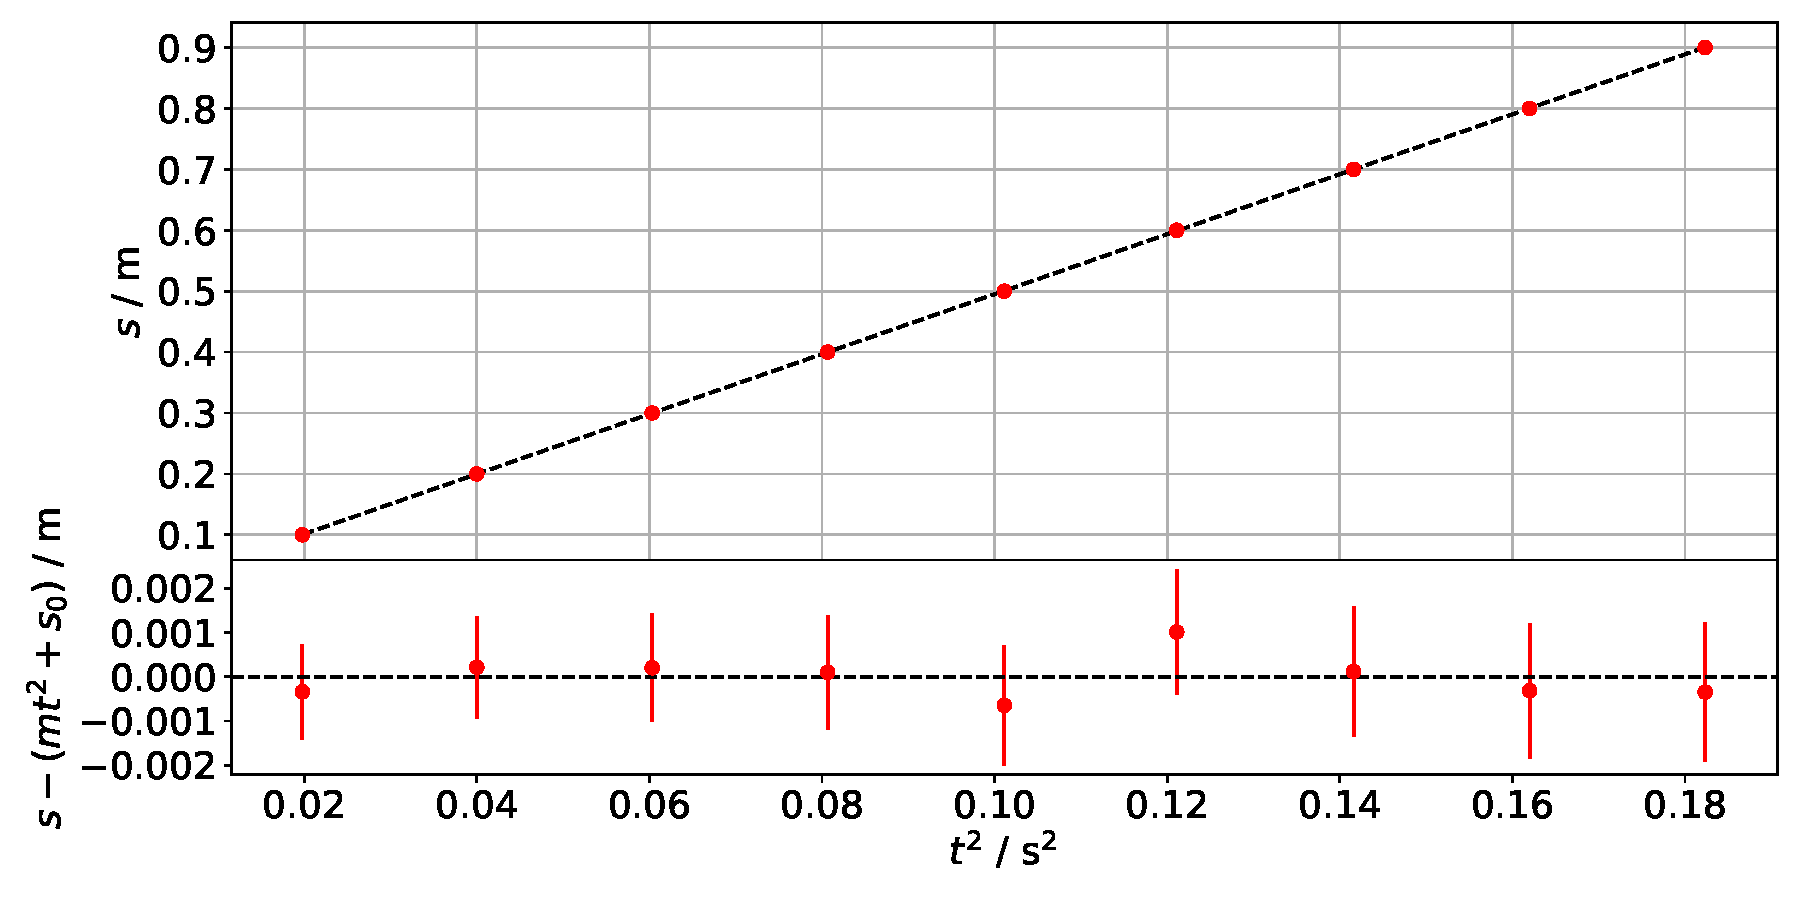
\includegraphics[width=\textwidth]{plots/regression_fF1.pdf}
	\caption{Residuenplot für den Digitalzähler}
	\label{ResDz}
\end{figure}

Der sehr schlechte Wert für $\chi^2/n_{df}$ spiegelt sich auch im Residuengraph wieder (Abb. \ref{ResDz}), wo alle Fehlerbalken deutlich die Nulllinie treffen. Zusammen führt dies zu dem Schluss, dass die Fehlerabschätzungen für $s$ und $t$ zu grob sind. Da wir jedoch keine bessseren Abschätzungen machen können, führen wir noch eine alternative Auswertung der Daten durch. Dazu berechnen wir für je zwei benachbarte Datenpunkte in unserem $s-t^2$-Diagramm die Steigung, wobei der erste Wert nicht verwendet wird. Für die Steigung gilt
$$m = \frac{s_{i+1}-s_i}{t_{i+1}^2-t_{i}^2}.$$
Dies liefert uns vier Schätzungen für die Steigung. Die Fehler werden mit einer Gaußschen Fehlerfortplanzung bestimmt. Diese liefert uns
$$\frac{\sigma_m^2}{m^2} = \frac{2}{(s_{i+1}-s_i)^2}\cdot\sigma_s^2 + \frac{4(t_{i+1}^2 + t_i^2)}{(t_{i+1}^2-t_i^2)^2}\cdot\sigma_t^2.$$
Anschließend werden die vier Steigungswerte mit ihren Unsicherheiten gewichtet gemittelt und innerer und äußerer Fehler des Mittelwertes bestimmt. Die Ergebnisse dieser Kalkulation sind in Tabelle \ref{tableAltAus} zu sehen. 

\begin{table}[h!]
\begin{center}
\begin{tabular}{c|c}
$m_1$ & $(4.921 \pm 0.083) \, \mathrm m / \mathrm s^2$ \\ 
$m_2$ & $(4.886 \pm 0.091) \, \mathrm m / \mathrm s^2$ \\
$m_3$ & $(4.879 \pm 0.099) \, \mathrm m / \mathrm s^2$ \\
$m_4$ & $(4.921 \pm 0.109) \, \mathrm m / \mathrm s^2$ \\
\hline
$\bar m$ & $4.902 \, \mathrm m / \mathrm s^2$ \\
$\sigma^{in}_{\bar m}$ & $0.047 \, \mathrm m / \mathrm s^2$ \\
$\sigma^{au}_{\bar m}$ & $0.011 \, \mathrm m / \mathrm s^2$
\end{tabular}
\caption{Alternative Auswertung der Daten}
\label{tableAltAus}
\end{center}
\end{table}
Aus dem Wert der Steigung ergibt sich dann die Schätzung für die Erdbeschleunigung
$$g = (9.80 \pm 0.09) \, \mathrm m / \mathrm s^2 .$$

\subsubsection{Messung mit dem Oszilloskop}

Die Messungen mit dem Oszilloskop sind in Tabelle \ref{tableOs} aufgeführt. 
\begin{table}[h!]
\begin{center}
\begin{tabular}{c|r|r|r|r|r|r|r|r|r}
$s$ / cm & 10 & 20 & 30 & 40 & 50 & 60 & 70 & 80 & 90 \\
\hline
$t$ / ms & 140.8 & 200.0 & 245.2 & 283.8 & 318.2 & 348.4 & 376.6 & 402.7 & 427.2 \\
\end{tabular}
\caption{Messreihe mit dem Oszilloskop}
\label{tableOs}
\end{center}
\end{table}

Die Genauigkeit der Zeitmessung mit dem Oszilloskop wird auf $\sigma_t = 0.1 \, \mathrm{ms}$ geschätzt. Wir führen wieder ein lineare Regression von $s$ über $t^2$ durch. Die Ergebnisse befinden sich in Tabelle \ref{tableReg2}.

\begin{table}[h!]
\begin{center}
\begin{tabular}{c|c|c}
$m$ & $s_0$ & $\chi^2/n_{df}$ \\
\hline
$(4.9123 \pm 0.0066) \, \mathrm m / \mathrm s^2$ & $(0.0035 \pm 0.0007) \, \mathrm m$ & $0.5$
\end{tabular}
\caption{Ausgabe der Regression}
\label{tableReg2}
\end{center}
\end{table}

Der Wert für $\chi^2/n_{df}$ deutet wieder auf eine zu grobe Fehlerabschätzung hin. Dies zeigt sich auch wieder im Residuenplot (Abb. \ref{ResOz}), wo fast alle Fehlerbalken die Nulllinie treffen.
\begin{figure}[h!]
	\centering
	%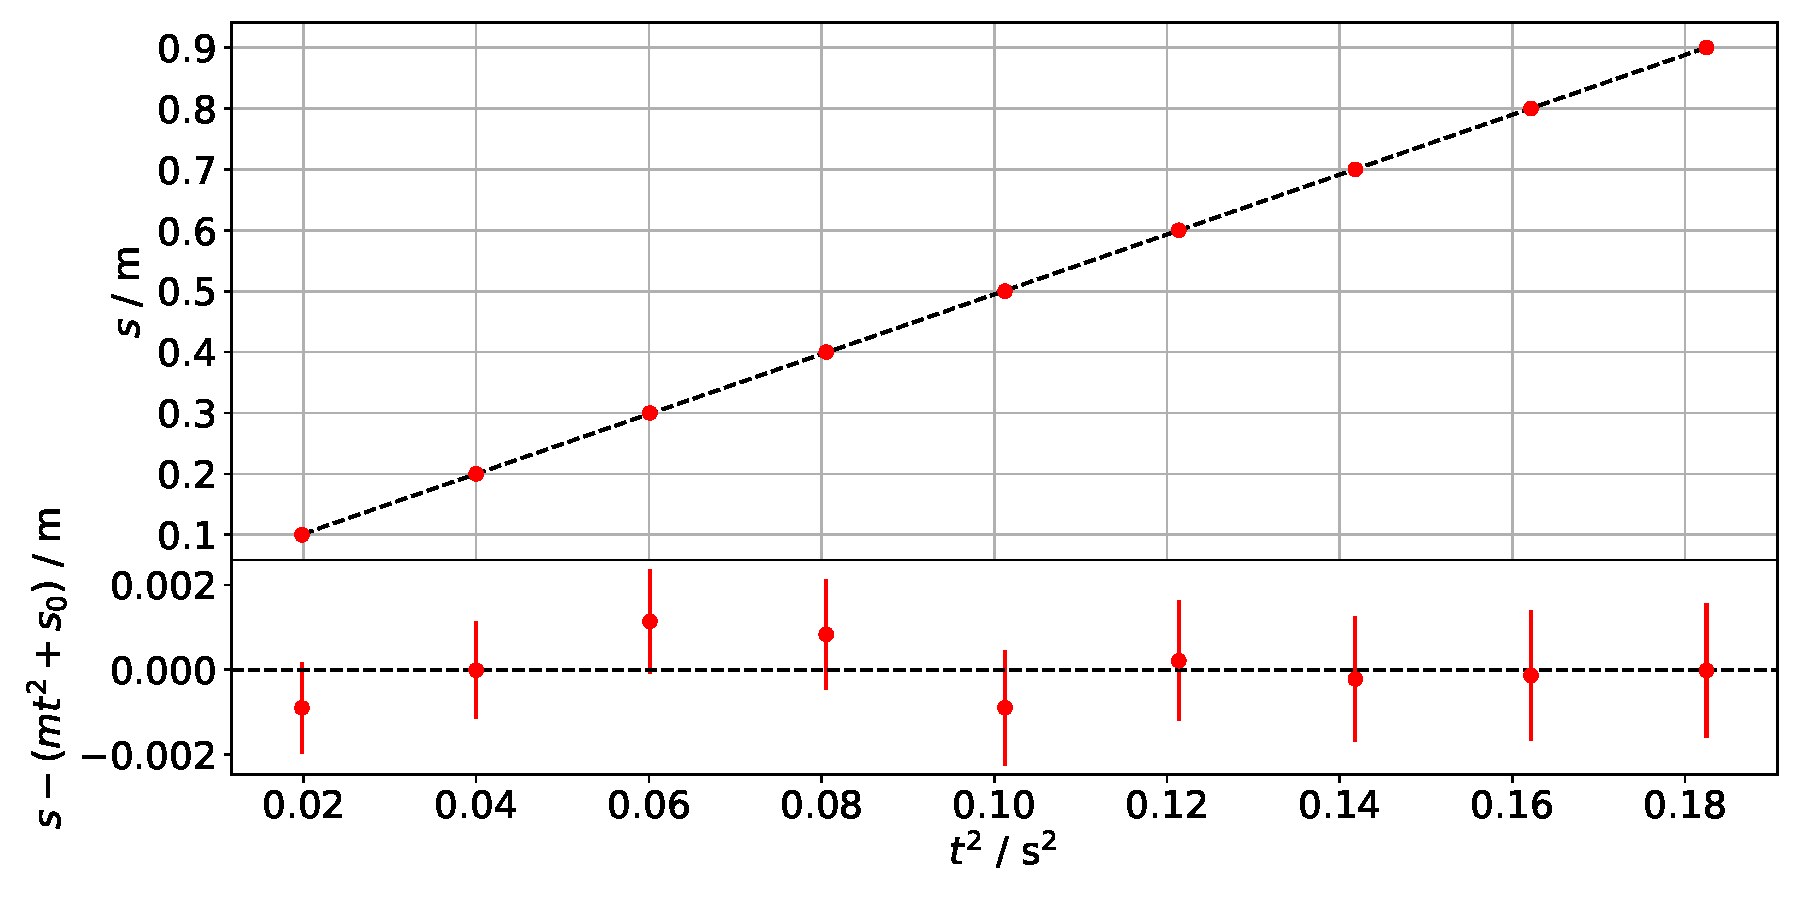
\includegraphics[width=\textwidth]{plots/regression_fF2.pdf}
	\caption{Residuenplot für das Oszilloskop}
	\label{ResOz}
\end{figure}
Trotzdessen verwenden wir die Ergebnisse dieser Regression, da die Anpassung deutlich besser ist, als im Falle des Digitalzählers. Aus der Steigung ermitteln wir folgende Schätzung für die Erdbeschleunigung
$$g = (9.824 \pm 0.013) \, \mathrm m / \mathrm s^2 .$$


\subsection{Fazit}

Wir haben nun zwei Schätzungen für die Erdbeschleunigung $g$ ermittelt. Wie im Fazit des zweiten Versuchs erläutert, verwenden wir als Literaturwert für die Erbeschleunigung in Aachen $g_L = 9.811 \, \mathrm m / \mathrm s^2$. 
Zur Bewertung der beiden Ergebnisse berechnen wir
\begin{align*}
\frac{|g_L-g_{Dz}|}{\sigma_{g_{Dz}}} &= 0.12 \\
\frac{|g_L-g_{Os}|}{\sigma_{g_{Os}}} &= 1
\end{align*}
In beiden Fällen liegen wir somit im $1\sigma$-Intervall. Zur Überprüfung der Übereinstimmung der beiden Werte untereinander berechnen wir noch
$$\frac{|g_{Os}-g_{Dz}|}{\sqrt{\sigma_{g_{Dz}}^2 + \sigma_{g_{Os}}^2}} \approx 0.03 \ll 1.$$
Die beiden Werten stimmen also im Rahmen der Unsicherheiten sehr gut überein. 


\newpage



\end{document}
